\documentclass[UTF8]{beamer}

\usetheme{Madrid}
\usecolortheme{seahorse}

\usepackage[english]{babel}
\usepackage{ctex}
\usepackage{algorithm,algorithmic}
\usepackage{tabularx}
\usepackage{graphicx}
\graphicspath{ {img/} }

\begin{document}

\title{SHTSC 2016 题目原文}
\frame{\titlepage}

%%%%%%%%%%%%%%%%%%%%%%%% Day 1 A %%%%%%%%%%%%%%%%%%%%%%%%

\begin{frame}{Problem 1. Robot}
[Touhou Contest by Nettle, Stage 1 A]

在幻想乡,东风谷早苗是以高达控闻名的高中生宅巫女。某一天,早苗终于入手了最新款的
钢达姆模型。作为最新的钢达姆,当然有了与以往不同的功能了,那就是它能够自动行走,厉害吧。

早苗的新模型可以按照输入的命令进行移动,命令包含“E”、“S”、“W”、“N”四种,
分别对应四个不同的方向,依次为东、南、西、北。执行某个命令时,它会向着对应
方向移动一个单位。作为新型机器人,自然不会只单单执行一个命令,它可以执行命令串。
对于输入的命令串,每一秒它会按照命令行动一次。而执行完命令串最后一个命令后,会自
动从头开始循环。在 0 时刻时早苗将钢达姆放置在了 (0,0) 的位置,并且输入了命令串。
她想要知道 $T$ 秒后钢达姆所在的位置坐标。

\end{frame}

\begin{frame}{Problem 1. Robot}

\textbf{输入}
\begin{itemize}
    \item 第 1 行:命令串 $S$
    \item 第 2 行:正整数 $T$
\end{itemize}
\textbf{输出}
\begin{itemize}
    \item 第 1 行:结束时的位置 $(X, Y)$
\end{itemize}

\begin{tabularx}{\textwidth}{|X|X|}
\hline
\texttt{\textbf{robot.in}} & \texttt{\textbf{robot.out}} \\ \hline
\texttt{NSWWNSNEEWN}\newline
\texttt{12}
&
\texttt{-1 3}
\\ \hline
\end{tabularx}
\newline
\begin{itemize}
    \item 60 pts: $|T| \leq 500\,000, |S| \leq 5\,000$
    \item 100 pts: $|T| \leq 2\,000\,000\,000, |S| \leq 5\,000$
\end{itemize}

\end{frame}

%%%%%%%%%%%%%%%%%%%%%%%% Day 1 B %%%%%%%%%%%%%%%%%%%%%%%%

\begin{frame}{Problem 2. Ice}
[Touhou Contest by Nettle, Stage 1 C]

在幻想乡,琪露诺是以笨蛋闻名的冰之妖精。某一天,琪露诺又在玩速冻青蛙,就是用冰把
青蛙瞬间冻起来。但是这只青蛙比以往的要聪明许多,在琪露诺来之前就已经跑到了河的对
岸。于是琪露诺决定到河岸去追青蛙。

\end{frame}

\begin{frame}{Problem 2. Ice}

小河可以看作一列格子依次编号为 0 到 $N$,琪露诺只能从编号小的格子移动到编号大的格子。
而且琪露诺按照一种特殊的方式进行移动,当她在格子 $i$ 时,她只会移动到 $i+L$ 到 $i+R$
中的一格。你问为什么她这么移动,这还不简单,因为她是笨蛋啊。每一个格子都有一个冰冻指数
$A_i$,编号为 0 的格子冰冻指数为 0 。当琪露诺停留在那一格时就可以得到那一格的冰冻指数
$A_i$。琪露诺希望能够在到达对岸时,获取最大的冰冻指数,这样她才能狠狠地教训那只青蛙。
但是由于她实在是太笨了,所以她决定拜托你帮它决定怎样前进。

开始时,琪露诺在编号 0 的格子上,只要她下一步的位置编号大于 $N$ 就算到达对岸。

\end{frame}

\begin{frame}{Problem 2. Ice}

\textbf{输入}
\begin{itemize}
    \item 第 1 行:三个整数 $N$,$L$,$R$
    \item 第 2 行:$N+1$ 个整数 $A_{0 \dots N}$
\end{itemize}
\textbf{输出}
\begin{itemize}
    \item 第 1 行:最大的冰冻指数
\end{itemize}

\begin{tabularx}{\textwidth}{|X|X|}
\hline
\texttt{\textbf{ice.in}} & \texttt{\textbf{ice.out}} \\ \hline
\texttt{5 2 3}\newline
\texttt{0 12 3 11 7 -2}
&
\texttt{11}
\\ \hline
\end{tabularx}
\newline
\begin{itemize}
    \item 60 pts: $N \leq 10\,000$
    \item 100 pts: $N \leq 200\,000, |A_i| \leq 1000, 1 \leq L \leq R \leq N$
\end{itemize}

\end{frame}

%%%%%%%%%%%%%%%%%%%%%%%% Day 1 C %%%%%%%%%%%%%%%%%%%%%%%%

\begin{frame}{Problem 3. Desired}

[BZOJ 3143] [HNOI 2013]

一个无向连通图,顶点从 1 编号到 $N$,边从 1 编号到 $M$。

小Z在该图上进行随机游走,初始时小Z在 1 号顶点,每一步小Z以相等的概率随机选择当前顶点的某条边,
沿着这条边走到下一个顶点,获得等于这条边的编号的分数。当小Z到达 $N$ 号顶点时游走结束,总分为所有获得的分数之和。
现在,请你对这 $M$ 条边进行编号,使得小Z获得的总分的期望值最小。

\end{frame}

\begin{frame}{Problem 3. Desired}

\textbf{输入}
\begin{itemize}
    \item 第 1 行:$N$,$M$
    \item 接下来 $M$ 行:每行描述一条无向边 $u, v$。
\end{itemize}
\textbf{输出}
\begin{itemize}
    \item 第 1 行:最小的期望值,保留 3 位小数
\end{itemize}

\begin{tabularx}{\textwidth}{|X|X|}
\hline
\texttt{\textbf{desired.in}} & \texttt{\textbf{desired.out}} \\ \hline
\texttt{3 3}\newline
\texttt{2 3}\newline
\texttt{1 2}\newline
\texttt{1 3}
&
\texttt{3.333}
\\ \hline
\end{tabularx}
\newline
\begin{itemize}
    \item 30 pts: $2 \leq N \leq 10$
    \item 100 pts: $2 \leq N \leq 500$
\end{itemize}

\end{frame}

%%%%%%%%%%%%%%%%%%%%%%%% Day 2 A %%%%%%%%%%%%%%%%%%%%%%%%

\begin{frame}{Problem 4. Pudding}

[BZOJ 1483] [HNOI 2009]

$N$ 个布丁摆成一行,每个布丁一开始有一种颜色 $A_i$。

进行 $M$ 次操作,每次操作是下列两种中的一种: \\
(1) 将某个颜色的布丁全部变成另一种颜色 \\
(2) 询问当前一共有多少段颜色,相同连续的颜色算作一段

\end{frame}

\begin{frame}{Problem 4. Pudding}

\textbf{输入}
\begin{itemize}
    \item 第 1 行:$N$,$M$
    \item 第 2 行:$N$ 个整数表示初始颜色 $A_{1 \dots N}$
    \item 接下来 $M$ 行:每行描述一次操作。 \\ “1 $X$ $Y$” 表示把颜色 $X$ 的布丁都变成颜色 $Y$,“2” 表示询问。
\end{itemize}
\textbf{输出}
\begin{itemize}
    \item 对于每个询问输出一行,表示当前颜色段数。
\end{itemize}

\end{frame}

\begin{frame}{Problem 4. Pudding}

\begin{tabularx}{\textwidth}{|X|X|}
\hline
\texttt{\textbf{pudding.in}} & \texttt{\textbf{pudding.out}} \\ \hline
\texttt{4 3}\newline
\texttt{1 2 2 1}\newline
\texttt{2}\newline
\texttt{1 2 1}\newline
\texttt{2}
&
\texttt{3}\newline
\texttt{1}
\\ \hline
\end{tabularx}
\newline
\begin{itemize}
    \item 60 pts: $2 \leq N \leq 1\,000$
    \item 100 pts: $2 \leq N \leq 100\,000$,颜色数 $\leq 10^6$
\end{itemize}

\end{frame}

%%%%%%%%%%%%%%%%%%%%%%%% Day 2 B %%%%%%%%%%%%%%%%%%%%%%%%

\begin{frame}{Problem 5. Num}

[不知道哪一场模拟赛的题……]

一个数字被称为好数字当它满足下列条件:

(1) 有 $2n$ 个数位,$n$ 是正整数\textbf{(允许有前导 0)}。

(2) 构成它的每个数位都在给定的数字集合 $S$ 中,$S \subseteq \{0,1,\dots,9\}$。

(3) 它前 $n$ 位之和与后 $n$ 位之和相等,或者它奇数位之和与偶数位之和相等

给出 $n$ 和 $S$,求合法的好数字的个数 mod 999983。

\end{frame}

\begin{frame}{Problem 5. Num}

\textbf{输入}
\begin{itemize}
    \item 第 1 行:正整数 $N$
    \item 第 2 行:数字集合 $S$
\end{itemize}
\textbf{输出}
\begin{itemize}
    \item 第 1 行:合法的好数字的个数 mod 999983。
\end{itemize}

\begin{tabularx}{\textwidth}{|X|X|}
\hline
\texttt{\textbf{num.in}} & \texttt{\textbf{num.out}} \\ \hline
\texttt{2}\newline
\texttt{0987654321}
&
\texttt{1240}
\\ \hline
\end{tabularx}
\newline
\begin{itemize}
    \item 20 pts: $n \leq 7$
    \item 100 pts: $n \leq 1\,000, |S| \leq 10$
\end{itemize}

\end{frame}

%%%%%%%%%%%%%%%%%%%%%%%% Day 3 A %%%%%%%%%%%%%%%%%%%%%%%%

\begin{frame}{Problem 7. Observer}

小 R 和 B 神正在玩一款游戏。这款游戏的地图由 $n$ 个点和 $n - 1$ 条无向边组成,
每条无向边连接两个点,且地图是连通的。换句话说,游戏的地图是一棵有 $n$ 个节点的树。

游戏中有一种道具叫做侦查守卫,当一名玩家在一个点上放置侦查守卫后,它可以监视这个点
以及与这个点的距离在 $d$ 以内的所有点。这里两个点之间的距离定义为它们在树上的距离,
也就是两个点之间唯一的简单路径上所经过边的条数。

在一个点上放置侦查守卫需要付出一定的代价,在不同点放置守卫的代价可能不同。现在小 R
知道了所有 B 神可能出现的位置,请你计算监视所有这些位置的最小代价。

\end{frame}

\begin{frame}{Problem 7. Observer}

\textbf{输入}
\begin{itemize}
    \item 第 1 行:两个正整数 $n$ 和 $d$,分别表示地图上的点数和侦查守卫的视野范围。
                    约定地图上的点用 1 到 $n$ 的正整数编号。
    \item 第 2 行:$n$ 个正整数,第 $i$ 个正整数表示在编号为 $i$ 的点放置侦查守卫的代价 $w_i$。保证 $w_i \leq 1000$。
    \item 第 3 行:一个正整数 $m$,表示 B 神可能出现的点的数量。保证 $m \leq n$。
    \item 第 4 行:$m$ 个正整数,分别表示每个 B 神可能出现的点的编号,从小到大不重复地给出。
    \item 接下来 $n - 1$ 行:每行包含两个整数 $u, v$,表示在编号为 $u$ 的点和编号为 $v$ 的点之间有一条无向边。
\end{itemize}
\textbf{输出}
\begin{itemize}
    \item 第 1 行:一个整数。表示监视所有 B 神可能出现的点所需要的最小代价。
\end{itemize}

\end{frame}

\begin{frame}{Problem 7. Observer}
\small{
\begin{tabularx}{\textwidth}{|X|X|}
\hline
\texttt{\textbf{observer.in}} & \texttt{\textbf{observer.out}} \\ \hline
\texttt{12 2}\newline
\texttt{8 9 12 6 1 1 5 1 2 8 10 6}\newline
\texttt{10}\newline
\texttt{1 2 3 5 6 7 8 9 10 11}\newline
\texttt{1 3}\newline
\texttt{2 3}\newline
\texttt{3 4}\newline
\texttt{4 5}\newline
\texttt{4 6}\newline
\texttt{4 7}\newline
\texttt{7 8}\newline
\texttt{8 9}\newline
\texttt{9 10}\newline
\texttt{10 11}\newline
\texttt{11 12}
&
\texttt{10}
\\ \hline
\end{tabularx}
}
\newline

\end{frame}

\begin{frame}{Problem 7. Observer}

\begin{tabularx}{\textwidth}{X|X|X|X} \hline
Case \# & $n$ & $d$ & Rmks \\ \hline \hline
1       & $\leq 20$       & $\leq 5$  & - \\ \hline
2, 3    & $\leq 500\,000$ & $= 1$     & - \\ \hline
4, 5    & $\leq 500\,000$ & $\leq 20$ & $n = m$ \\ \hline
6, 7, 8 & $\leq 10\,000$  & $\leq 20$ & - \\ \hline
9, 10   & $\leq 500\,000$ & $\leq 20$ & - \\ \hline
\end{tabularx}

\end{frame}

%%%%%%%%%%%%%%%%%%%%%%%% Day 3 B %%%%%%%%%%%%%%%%%%%%%%%%

\begin{frame}{Problem 8. Square}

上帝说,不要圆,要方,于是便有了这道题。

由于我们应该方,而且最好能够尽量方,所以上帝派我们来找正方形。
上帝把我们派到了一个有 $N$ 行 $M$ 列的方格图上,图上一共有 $(N + 1) \times (M + 1)$ 个
格点,我们需要做的就是找出这些格点形成了多少个正方形(换句话说,正方形的四个顶点都是格点)。

但是这个问题对于我们来说太难了,因为点数太多了,所以上帝删掉了这 $(N + 1) \times (M + 1)$
中的 $K$ 个点。既然点变少了,问题也就变简单了,那么这个时候这些格点组成了多少个正方形呢?

\end{frame}

\begin{frame}{Problem 8. Square}

\textbf{输入}
\begin{itemize}
    \item 第 1 行:三个整数 $N$,$M$,$K$,代表棋盘的行数、列数和不能选取的顶点个数。
                    保证 $N, M \leq 1$,$K \leq (N + 1) \times (M + 1)$。
    \item 接下来 $K$ 行:每行两个正整数 $X$,$Y$,代表第 $X$ 行第 $Y$ 列的格点被删掉了。
                    保证 $0 \leq X \leq N, 0 \leq Y \leq M$,且不会出现重复的格点。
                    约定每行的格点从上到下依次用整数 0 到 $N$ 编号,每列的格点依次用 0 到 $M$ 编号。
\end{itemize}
\textbf{输出}
\begin{itemize}
    \item 第 1 行:一个正整数,代表正方形个数对 100000007($10^8 + 7$)取模之后的数值。
\end{itemize}

\end{frame}

\begin{frame}{Problem 8. Square}
\only<1>{
\small{\begin{tabularx}{\textwidth}{|X|X|}
\hline
\texttt{\textbf{square.in}} & \texttt{\textbf{square.out}} \\ \hline
\texttt{2 2 4}\newline
\texttt{1 0}\newline
\texttt{1 2}\newline
\texttt{0 1}\newline
\texttt{2 1}
&
\texttt{1}
\\ \hline
\end{tabularx}}
\newline
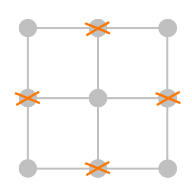
\includegraphics[scale=0.85]{square-sample1.png}
\newline
*如图所示,我们删掉了其中的四个格点,那么剩下的唯一的正方形便是最大的 $2 \times 2$ 的正方形了。}

\only<2>{
\begin{tabularx}{\textwidth}{|X|X|}
\hline
\texttt{\textbf{square.in}} & \texttt{\textbf{square.out}} \\ \hline
\texttt{7 10 5}\newline
\texttt{2 3}\newline
\texttt{1 5}\newline
\texttt{6 2}\newline
\texttt{3 5}\newline
\texttt{2 6}
&
\texttt{729}
\\ \hline
\end{tabularx}
\newline}

\only<3>{
\begin{tabularx}{\textwidth}{|X|X|}
\hline
\texttt{\textbf{square.in}} & \texttt{\textbf{square.out}} \\ \hline
\texttt{2 2 4}\newline
\texttt{0 0}\newline
\texttt{2 2}\newline
\texttt{0 2}\newline
\texttt{2 0}
&
\texttt{1}
\\ \hline
\end{tabularx}
\newline
*还剩下一个边长为 $\sqrt 2$ 的正方形。}

\end{frame}

\begin{frame}{Problem 8. Square}

\begin{tabularx}{\textwidth}{X|X|X} \hline
Case \# & $N, M$ & $K$ \\ \hline \hline
1, 2   & $\leq 5$    & $\leq 25$            \\ \hline
3, 4   & $\leq 50$   & $\leq 50$            \\ \hline
5, 6   & $\leq 10^6$ & $= 0$                \\ \hline
7, 8   & $\leq 10^6$ & $\leq 50$            \\ \hline
9, 10  & $\leq 10^6$ & $\leq 200$           \\ \hline
11, 12 & $\leq 10^3$ & $\leq 2 \times 10^3$ \\ \hline
13\textasciitilde 20 & $\leq 10^6$ & $\leq 2 \times 10^3$ \\ \hline
\end{tabularx}

\end{frame}

%%%%%%%%%%%%%%%%%%%%%%%% Day 3 C %%%%%%%%%%%%%%%%%%%%%%%%

\begin{frame}{Problem 9. Mark / 成绩比较}

THU 的 G 系中有许许多多的大牛,比如小 R 的室友 B 神。B 神已经厌倦了与其他的同学比较 GPA
(Grade Point Average,平均学分绩),他只在意 G 系中共有多少同学被他“碾压”。

B 神声称,在 G 系共有 $k$ 位同学被他碾压。

同是 G 系大牛的 D 神则认为 B 神在吹牛,他查到了 B 神每门必修课在 G 系的排名。
他用了 173 毫秒的时间就计算出了有多少种情况使得 B 神所说的话成立。
现在他想考考聪明的你,看你是否也能求出这个情况数。

\end{frame}

\begin{frame}{Problem 9. Mark / 成绩比较}

G 系共有 $n$ 位同学,$m$ 门必修课。这 $n$ 位同学的编号为 0 到 $n - 1$ 的整数,
其中 B 神的编号为 0 号。这 $m$ 门必修课编号为 0 到 $m - 1$ 的整数。

如果在每门课上 A 获得的成绩均小于等于 B 获得的成绩,则称 A 被 B 碾压。
在 B 神的说法中,G 系共有 $k$ 位同学呗碾压(不包括他自己),而其他 $n - k - 1$
名同学则没有被他碾压。

\end{frame}

\begin{frame}{Problem 9. Mark / 成绩比较}

D 神查到了 B 神每门必修课的排名。这里的排名是指,如果 B 神某门课的排名为 $r$,则表示
有且仅有 $r - 1$ 位同学这门课的分数\textbf{大于} B 神的分数,有且仅有 $n - r$
位同学这门课的分数\textbf{小于等于} B 神(不包括他自己)。

我们需要求出全系所有同学每门必修课得分的情况数,使其既能满足 B 神的说法,也能符合
D 神查到的排名。这里两种情况不同当且仅当有任意一位同学在任意一门课上获得的分数不同。

你不需要像 D 神那么厉害,你只需要计算出情况数模 $10^9 + 7$ 的余数就可以了。

\end{frame}

\begin{frame}{Problem 9. Mark / 成绩比较}

\textbf{输入}
\begin{itemize}
    \item 第 1 行:三个正整数 $n, m, k$,分别表示 G 系的同学数量(包括 B 神)、必修课的数量和被 B 神碾压的同学数量。
    \item 第 2 行:$m$ 个正整数,依次表示每门课的最高分 $u_i$。
    \item 第 3 行:$m$ 个正整数,依次表示 B 神在每门课上的排名 $r_i$。保证 $1 \leq r_i \leq n$。

    数据保证至少有 1 种情况使得 B 神说的话成立。
\end{itemize}
\textbf{输出}
\begin{itemize}
    \item 一行一个正整数,表示满足条件的情况数模 $10^9 + 7$ 的余数。
\end{itemize}

\end{frame}

\begin{frame}{Problem 9. Mark / 成绩比较}

\begin{tabularx}{\textwidth}{|X|X|}
\hline
\texttt{\textbf{mark.in}} & \texttt{\textbf{mark.out}} \\ \hline
\texttt{3 2 1}\newline
\texttt{2 2}\newline
\texttt{1 2}
&
\texttt{10}
\\ \hline
\end{tabularx}
\newline

\begin{tabularx}{\textwidth}{|X|X|}
\hline
\texttt{\textbf{mark.in}} & \texttt{\textbf{mark.out}} \\ \hline
\texttt{5 3 2}\newline
\texttt{4 3 2}\newline
\texttt{2 1 2}
&
\texttt{54096}
\\ \hline
\end{tabularx}
\newline

\end{frame}

\begin{frame}{Problem 9. Mark / 成绩比较}

\begin{tabularx}{\textwidth}{X|X|X|X} \hline
Case \# & $n$ & $m$ & $u_i$ \\ \hline \hline
1    & $\leq 3$   & $\leq 3$   & $\leq 4$    \\ \hline
2    & $\leq 3$   & $\leq 10$  & $\leq 100$  \\ \hline
3    & $\leq 3$   & $\leq 100$ & $\leq 10^9$ \\ \hline
4, 5 & $\leq 5$   & $\leq 100$ & $\leq 10^9$ \\ \hline
6, 7 & $\leq 50$  & $\leq 50$  & $\leq 50$   \\ \hline
8 \textasciitilde 10 & $\leq 100$ & $\leq 100$ & $\leq 10^9$ \\ \hline
\end{tabularx}

\end{frame}

%%%%%%%%%%%%%%%%%%%%%%%% Day 4 A %%%%%%%%%%%%%%%%%%%%%%%%

\begin{frame}{Problem 10. Ptree / 黑暗前的幻想乡}

四年一度的幻想乡大选开始了,最近幻想乡最大的问题是很多来历不明的妖怪涌入了幻想乡,
扰乱了幻想乡昔日的秩序。但是幻想乡的建制派妖怪(人类)博丽灵梦和八云紫等人
整日高谈所有妖怪平等,幻想乡多元化等等,对于幻想乡目前棉铃的种种大问题却给不出合理的解决方案。

风见幽香是幻想乡里少有的意识到了问题严重性的大妖怪。她这次勇敢地站了出来参加幻想乡大选,
提出包括在幻想乡边境建墙(并让人类出钱),大力开展基础设施建设挽回失业率等一系列方案,
称为了大选年出人意料的黑马并顺利地当上了幻想乡的大统领。

\end{frame}

\begin{frame}{Problem 10. Ptree / 黑暗前的幻想乡}

幽香上台以后,第一项措施就是要修建幻想乡的公路。
幻想乡一共有 $n$ 个城市,之前原来没有任何路。幽香向选民承诺要减税,所以她打算只修
$n - 1$ 条公路将这些城市连接起来。但是幻想乡有正好 $n - 1$ 个建筑公司,每个建筑公司都想
在修路地过程中获得一些好处。

虽然这些建筑公司在选举前没有给幽香钱,幽香还是打算和他们搞好关系,因为她还指望他们帮她建墙。
所以她打算让每个建筑公司都负责一条路来修。

\end{frame}

\begin{frame}{Problem 10. Ptree / 黑暗前的幻想乡}

每个建筑公司都告诉了幽香自己有能力负责修建的路是哪些城市之间的。所以幽香打算 $n - 1$ 条
能够连接幻想乡所有城市的边,然后每条边都交给一个能够负责该边的建筑公司修建,并且
每个建筑公司都恰好修建一条边。

幽香现在想要知道一共有多少种可能的方案呢?两个方案不同当且仅当它们要么修的边的集合不同,
要么边的分配方式不同。

\end{frame}

\begin{frame}{Problem 10. Ptree / 黑暗前的幻想乡}

\textbf{输入}
\begin{itemize}
    \item 第 1 行:一个整数 $n$,表示城市个数。
    \item 接下来 $n - 1$ 行:第 $i$ 行表示 第 $i$ 个建筑公司可以修建的路的列表。
        \begin{itemize}
            \item 以一个非负数 $m_i$ 开头,表示其可以修建 $m_i$ 条路;
            \item 接下来有 $m_i$ 对数,每对数表示一条边的两个短点。其中不会出现重复的边,也不会出现自环。
        \end{itemize}
\end{itemize}
\textbf{输出}
\begin{itemize}
    \item 一行一个整数,表示所有可能的方案数对 $10^9 + 7$ 取模的结果。
\end{itemize}

\small{\begin{tabularx}{\textwidth}{|X|X|}
\hline
\texttt{\textbf{ptree.in}} & \texttt{\textbf{ptree.out}} \\ \hline
\texttt{4}\newline
\texttt{2 3 2 4 2}\newline
\texttt{5 2 1 3 1 3 2 4 1 4 3}\newline
\texttt{4 2 1 3 2 4 1 4 2}
&
\texttt{17}
\\ \hline
\end{tabularx}}
\newline

\end{frame}

\begin{frame}{Problem 10. Ptree / 黑暗前的幻想乡}

\begin{tabularx}{\textwidth}{X|X} \hline
Case \# & $n$ \\ \hline \hline
1, 2                 & $\leq 5$  \\ \hline
3 \textasciitilde 5  & $\leq 8$  \\ \hline
6                    & $\leq 10$ \\ \hline
7 \textasciitilde 10 & $\leq 17$ \\ \hline
\end{tabularx}

\end{frame}

%%%%%%%%%%%%%%%%%%%%%%%% Day 4 B %%%%%%%%%%%%%%%%%%%%%%%%

\begin{frame}{Problem 11. Rand}

你的面前有 $n$ 个数排成一行,分别为 $a_1, a_2, \dots, a_n$。你打算在每相邻的两个
$a_i$ 和 $a_{i+1}$ 间都插入一个加号、减号或者乘号。那么一共有 $3^{n-1}$ 种可能的表达式。

你对所有可能的表达式的值的和非常感兴♂趣。但这毕竟太简单了,所以你海打算支持一个修改操作,
可以修改某个 $a_i$ 的值。

你能够编写一个程序对每个修改都输出修改完之后所有可能表达式的和吗?注意,修改是永久的,也就是说
每次修改都是在上一次修改的基础上进行,而不是在最初的表达式上进行。

\end{frame}

\begin{frame}{Problem 11. Rand}

\textbf{输入}
\begin{itemize}
    \item 第 1 行:两个正整数 $n$ 和 $Q$,为数的个数和询问的个数。
    \item 第 2 行:$n$ 个非负整数,依次表示 $a_1, a_2, \dots, a_n$。
    \item 接下来 $Q$ 行:每行两个整数 $t$ 和 $v$,表示要将 $a_t$ 修改为 $v$,其中 $1 \leq t \leq n$。
\end{itemize}
\textbf{输出}
\begin{itemize}
    \item 对于每个修改输出一行,包含一个整数,表示修改之后所有可能表达式的和,对 $10^9 + 7$ 取模。
\end{itemize}

\end{frame}

\begin{frame}{Problem 11. Rand}

\begin{tabularx}{\textwidth}{|X|X|}
\hline
\texttt{\textbf{rand.in}} & \texttt{\textbf{rand.out}} \\ \hline
\texttt{5}\newline
\texttt{9384 887 2778 6916 7794}\newline
\texttt{2 8336}\newline
\texttt{5 493}\newline
\texttt{3 1422}\newline
\texttt{1 28}\newline
\texttt{4 60}
&
\texttt{890543652}\newline
\texttt{252923708}\newline
\texttt{942282590}\newline
\texttt{228728040}\newline
\texttt{608998099}
\\ \hline
\end{tabularx}
\newline

\end{frame}

\begin{frame}{Problem 11. Rand}

\begin{tabularx}{\textwidth}{X|X} \hline
Case \# & $n, Q$ \\ \hline \hline
1, 2                 & $\leq 10$       \\ \hline
3 \textasciitilde 5  & $\leq 1\,000$   \\ \hline
6 \textasciitilde 10 & $\leq 100\,000$ \\ \hline
\end{tabularx}

所有的 $a_i$、$v$ 满足 $1 \leq a_i, v \leq 10^4$。

\end{frame}

\end{document}
